%
% File acl2018.tex
%
%% Based on the style files for ACL-2017, with some changes, which were, in turn,
%% Based on the style files for ACL-2015, with some improvements
%%  taken from the NAACL-2016 style
%% Based on the style files for ACL-2014, which were, in turn,
%% based on ACL-2013, ACL-2012, ACL-2011, ACL-2010, ACL-IJCNLP-2009,
%% EACL-2009, IJCNLP-2008...
%% Based on the style files for EACL 2006 by
%%e.agirre@ehu.es or Sergi.Balari@uab.es
%% and that of ACL 08 by Joakim Nivre and Noah Smith

\documentclass[11pt,a4paper]{article}
\usepackage[hyperref]{acl2018}
\usepackage{times}
\usepackage{latexsym}
\usepackage{mathtools}
\usepackage{amssymb}
\usepackage{url}
\usepackage{graphicx}
\graphicspath{ {images/} }

\aclfinalcopy % Uncomment this line for the final submission
%\def\aclpaperid{***} %  Enter the acl Paper ID here

%\setlength\titlebox{5cm}
% You can expand the titlebox if you need extra space
% to show all the authors. Please do not make the titlebox
% smaller than 5cm (the original size); we will check this
% in the camera-ready version and ask you to change it back.

\title{Second Project of the Natural Language Processing Course}

\author{Luca Di Liello \\
	University of Trento\\
	{\tt luca.diliello@studenti.unitn.it }
}


\begin{document}
\maketitle

\begin{abstract}

This document contains the instructions to prepare, implement and test a simple bot, which will allow users to search for a restaurant and make reservations using the voice. The program has been developed using the open-source python libraries \textit{RasaNLU}, \textit{RasaCore}, \textit{SpeechRecognition} (with Google API's) and \textit{pyttsx3}. RasaNLU is a natural language understanding framework to extract intents and entities from sentences while RasaCore uses this informations to choose the best next action to be executed. Both are written in Python given the giant number of machine learning tools available for this language and both can be run in a ``standalone'' mode or in server mode. SpeechRecognition is a simple library that allows to use the Google Speech Recognition service and to easily transform speech into text. Finally, we will use pyttsx3 to transform text in speech but without using external services.

\end{abstract}

\section{Credits}

The software and the techniques showed in this document were learned during the LUS course by professor Giuseppe Riccardi and professor Evgeny Stephanov. The core of the software is powered by the open-source libraries RasaNLU and RasaCore which permitted a much faster development of the project thanks to the powerful primitives to extract intent and entities from sentences and to take decision on what to do next. The TTS and STT tasks were allowed by the other two, previous mentioned, libraries pyttsx3 and SpeechRecognition.

\section{Introduction}

This document will touch four big tasks of the Human-Machine Spoken Dialog cycle, that are speech recognition,  natural language understanding, dialogue management the speech generation. The language generation part will not be treated as it's pretty complicated and still not generally a completely solved problem. First, we will briefly speak about the methods we used to transform speech in text and vice-versa, then there will be a deeper treatment of the two Rasa frameworks, with our implementations and tests.

\subsection{The Human Machine Spoken Dialog}

The Human Machine Spoken Dialog is the set of all components that, together, allow people to speak with a machine and do some tasks. The components are executed in series as a cycle, each component taking as input the output of the previous one.

\begin{itemize}
\item Speaker
\item Automatic Speech Recognition
\item Natural Language Understanding
\item Dialogue Manager
\item Language Generation
\item Text to Speech Synthesis
\item Speaker
\end{itemize}

The \textit{Automatic Speech Recognition} and the \textit{Text to Speech Synthesis} are the components that have to interact directly with the user. The first has to take in input a discrete electric signal representing sound waves and convert it to a sequence of tokens. There are many online services (Google first) that help doing this task easily.
After having converted speech in text, the next step consists in the extraction of intents and entities from the input sentence. This task is called \textit{Natural Language Understanding}. Intents are a finite set of what the user wants to do, for example a request or a command. Better results can be obviously obtained trying to use one intent for each sentence and trying to keep the set of possible intents small. On the other side entities are the important informations that have to be extracted from the sentence and that have to be used by the machine. For example, the sentence ``please search for an Italian restaurant in London" contains two entities: the type of cuisine and the location of the restaurant. In this case the intent was to do a research of restaurants.
Once intents and entities have been correctly extracted, they are used by the \textit{Dialogue Manager} to take decisions on what the bot should do next. Dialogue Managers can be seen as routers: they take in input intents and entities and have to decide which action the bot should execute. For better performances they often receive in input a record of the past interactions too. What are actions? Actions are functions that use all the previous informations to create a response for the user. They often can query a database or make online searches. The output of the action is a sequence of informations that has to be sent back to the user, but are not yet human friendly. The transduction of information in sentences for the user is done by the \textit{Language Generation} module. This task is one of the most difficult and this project will not cover how to create such a module, it will only generate predefined sentences and use simple templates.
Finally, once the sentence has been created, a \textit{Text to Speech Synthesizer} provides the functionalities to transform them in sound waves that can be understood by humans, trying to emulate all the human behaviours while speaking, for example doing little pauses between different sentences, changes of tones, variations of the pitch and the correct use of accents. The cycle will then restart if the user says something else.
 
\subsection{RasaNLU and RasaCore}

Rasa is an open-source project that develops two powerful frameworks to do \textit{Natural Language Understanding} and \textit{Dialogue Management}. 

\subsubsection{RasaNLU}

RasaNLU allows to train a model for the extraction of entities and the classification intents. It uses the power of different existent ML and NLP libraries like Spacy and TensorFlow. Each model can be build as the combination of different layers that will be processed in pipeline. For example, the default \textit{spacy\_sklearn} pipeline will use 7 different layers, each one with a different task like tokenisation and featurization. It can reach quite perfect performances in entities extraction and intent classification. Broadly, it works better if sentences are not too long and there are no more than 3-4 entities per sentence. Intents are good classified too if they are not too many and if sentence are not too long.

\subsubsection{RasaCore}

RasaCore is a framework to decide the best action to execute given the story of the dialogue and the last intent/entities from the user. The core of the framework are the policies, which are trained to predict the next action to execute based on the history of the dialogue and the last user interaction. For each action a probability is computed and the one with the highest is launched. Policies can use neural networks, SVM and lots of other machine learning tools to improve their performances and should be trained through stories. A story is a sequence of user intents and bot actions describing a dialogue from beginning to end, often enriched with entities and other data. The additive data are contained in data structures called slots, which are filled and changed during the conversation. Slots basically keep track of the conversation and are automatically updated when entities are extracted. There is the possibility to set them manually through events too.

\section{Datasets Overview}

There are 2 main datasets, one to train the Natural Language Understanding model and one for the Dialogue Manager.

\subsection{Franken Data}

The dataset for the NLU task is called Franken Data and contains 1977 sentences. For each sentence, the corresponding intent and entities are given. There are only six possible intents, that are: 

\begin{itemize}
\item \textit{inform}, that appears 1014 times
\item \textit{thankyou}, that appears 589 times
\item \textit{affirm}, that appears 260 times
\item \textit{deny}, that appears 85 times
\item \textit{greet}, that appears 13 times
\item \textit{request\_info}, that appears 16 times
\end{itemize}

The sentences have a very low average length of 4.4 words, and this will lead to very satisfying results in the accuracy of the RasaNLU model.
The entities are not so many, with an average of only 0.65 entities extracted from each sentence (1293 in total). There are lot of very simple sentences like \textit{ok great} or \textit{perfect thank you} that do not contain entities at all while some others have up to 4 entities and are longer (up to 22 words), especially those whose intent is to inform or request for informations. For each entity there are information about the part of the sentence in which it was found, to help the algorithm perform better. There are 5 different categories of entities:

\begin{itemize}
\item \textit{cuisine}, with 70 different specialities (573 total instances)
\item \textit{price}, with 6 different ranges (354 total instances)
\item \textit{location}, with 9 different places (338 total instances)
\item \textit{people}, meaning the number of sits to book (12 total instances)
\item \textit{info}, address or phone number (16 total instances)
\end{itemize}

As for the intents, the distribution of different entities is not uniform, and this will lead to situations in which some not popular entities will not be correctly extracted. 

\subsection{bAbi stories}

The bAbi story dataset is a collection of stories developed by Facebook. Our version contains 1000 different stories about the process of booking a table in a restaurant. There is a common pattern that can be identified easily looking at the dataset, that is:

\begin{itemize}
\item The user greets
\item Bot ask how can help
\item User ask for a restaurant with some requirements
\item Bot keeps asking missing info
\item User gives info requested by the bot
\item Bot shows some results and ask the user if they are ok
\item User says if they are fine, otherwise Bot propose other solutions
\item User thanks
\item Regards
\end{itemize}

The average length of the conversation, including both user requests and Bot responses, is of 25 actions and intents. There are cases in which the Bot executes more than one action in a row, especially proposing restaurants or confirming an info and then requesting something else. In each story, there are intents of the user with some entities in attachment, to better simulate a real conversation. As showed in the story pattern before, all the conversations start with greetings and ends with regards but there is no limit to the number of times a user can choose to change some info for the query or ask for other results.

\section{Techniques}

\subsection{Speech2Text \& Text2Speech}

For the conversion on speech in text, we used the \textit{Speech Recognition} library, which allows to use Google's speech recognition services without having to implement particular algorithms. This requires an active internet connection while using the bot with speech interaction enabled. Moreover, a good microphone with noise reduction is recommended in order to obtain a better voice recognition.
There are studies that shows that the Google Speech Recognition service work very well. Most of the (rare) errors are due to delays in the internet connection \cite{speech_study}.
For the opposite task, we used the library pyttsx3, a porting of the original library pyttsx on Python3. This works pretty well on all operating systems, especially with the ones with good speakers and in few lines of code is possible to hear our machine speaking.

\subsection{Rasa NLU}

The Rasa NLU model has to be set up through a config file, in which we have to specify two important parameters: the human language of the LUS and the pipeline of layers that will compose the model \cite{rasa_nlu}. The first field is very simple and only requires one string like \textit{en}, \textit{it} or \textit{de}. We used English and downloaded the large version of the spacy dataset, called \textit{en\_core\_web\_lg}, to achieve better performances but paying with lower training and test speed.

We trained and evaluated three different pipeline templates: 
\begin{itemize}
\item Spacy + Scikit-Learn
\item Mitie
\item Mitie + Scikit-Learn
\end{itemize}

Each of the three templates is built of different layers that do different tasks. There are layers that initialises the NLU model, like \textit{nlp\_spacy} and \textit{nlp\_mitie} that should be put at the beginning to be used by the other components. Then there are layers that do not output nothing but their functions are used by next components, for example ngram algorithms or spacy featurizers. Finally, at the end of the pipeline there are layers whose task is to extract entities and intent from the sentence, using, if possible, previous layers help to improve performances \cite{pipeline}.
Each component of the pipeline can be tuned with lots of parameters, going to modify for example the performances of the internal neural network, of the support vector machine or of the conditional random field algorithm. While there are complex entity extractors and intent recognisers that uses NN or CRF, there are others very simple and fast which use simple regular expressions and string similarity functions, but their performances are not competitive.

\subsection{Rasa Core}

The Rasa Core module requires a domain file in which there will be specifications about slots, entities, intents, templates and actions \cite{rasa_core}. One more advanced thing that has to be specified directly in the Python code when training a model is the policies it should use to take decisions. Built-in examples use some default policies like \textit{MemoizationPolicy} and \textit{KerasPolicy}. There is also the possibility to extend the default Policy class to create new custom policies that can be more specific for certain tasks and so perform better.
Actions, like policies, can be created by programmers simply extending some of the existent Action classes. There are few important methods they have to implement, first of the one that is called when an Action is executed. Furthermore, Rasa Core provides built-in action called \textit{utter\_actions} that performs simple tasks like sending a message back to the user.
Our Bot will be very similar to the example of the restaurant but with some improvements:
\begin{itemize}
\item More different possible responses of utter actions to avoid the bot repeating always the same sentences.
\item Integration with a \textit{mongodb} database with lots of restaurants to simulate a real search.
\item A Form Actions to fill all the tracker slots semi-automatically.
\end{itemize}

\subsubsection{FormAction}
Form Actions are a new type of actions, available from version 0.9.0. They are very useful to collect some different data from the user without having to launch different actions and to call the policies several times. Basically, a Form Action will end only when all the slots defined in that action are filled with user data. It will manage the dialogue autonomously keeping asking the user for missing info, until all the requirements are satisfied.

\section{Test and Results}

All the test has been launched on a i7 processor at 3.3GHz with 4 active cores. Note that the Rasa framework does not support multithreading but all ML layers like Tensorflow and Spacy does.

\subsection{Rasa NLU}

As mentioned, the Franken Data file, contains 1977 samples with only 6 different intents and 5 entities classes. This leads to very good results, even with the faster pipeline. These are the results of the 3 different pipelines, the first using the sklearn-spacy template, the second using the standard mitie template and the third using mitie plus sklearn. The test has been done using cross-validation with 5 folds on the Franken dataset and are showed in Figure \ref{fig:results1}.

\begin{figure}
  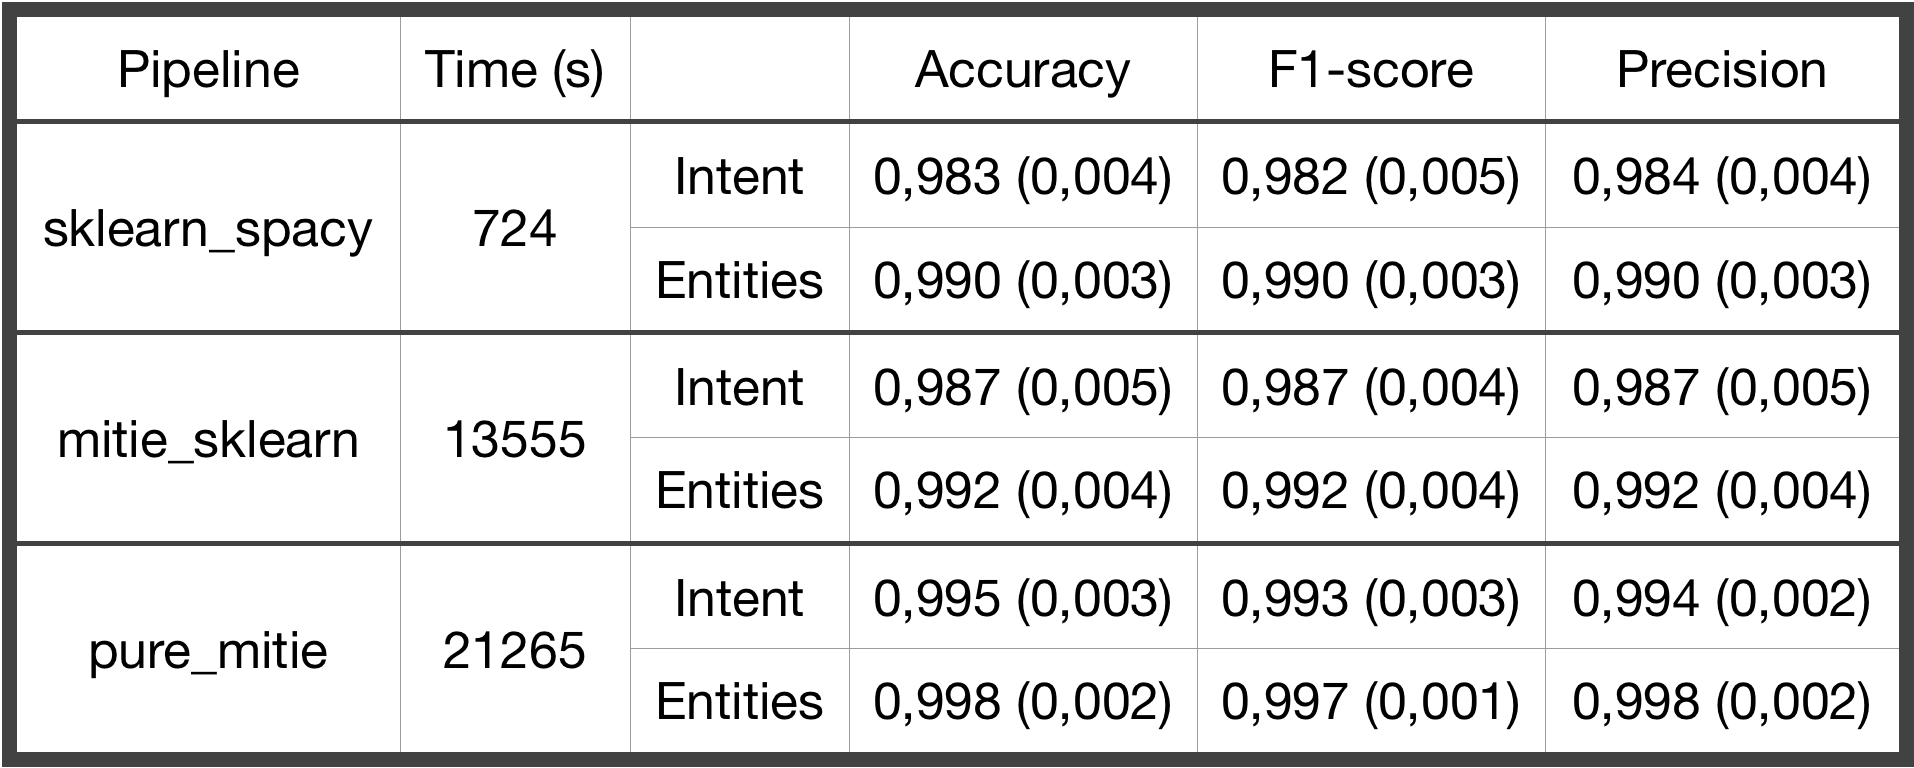
\includegraphics[scale=0.23]{nlu_results}
  \caption{NLU results}
  \label{fig:results1}
\end{figure}

The number in brackets is the standard deviation of the results during cross-validation. All three pipelines perform very well, with an F1-score always over 0.98. However, the interesting case is the sklearn\_spacy pipeline because, even if it performs a little worse than the others, it is 20 or 30 times faster. The time column shows how many seconds elapsed since the beginning of the test, so it includes both the time spent training the algorithm and the time needed to test it. The few errors in the entities extraction were mainly due to the \textit{north american} cuisine and the \textit{north} location, because sometimes happened that the second was extracted instead of the first. With regards to the intent classification, the few errors we noticed were on some \textit{request\_info} being classified as \textit{affirm} intents.  

\subsection{Rasa Core}

First of all, the stories dataset has been randomly shuffled and divided in training and test sets with dimensions of 70\% and 30\% w.r.t. the original one. Then the following combinations of policies has been trained and tested:

\begin{itemize}
\item MemoizationPolicy with max history 3
\item MemoizationPolicy with max history 5
\item AugmentedMemoizationPolicy
\item RestaurantPolicy
\item KerasPolicy
\item FallbackPolicy
\item FallbackPolicy with a core threshold of 0.5
\item SklearnPolicy
\item MemoizationPolicy with max history 3 and RestaurantPolicy
\item AugmentedMemoizationPolicy and RestaurantPolicy
\item MemoizationPolicy and KerasPolicy
\item AugmentedMemoizationPolicy and KerasPolicy
\item MemoizationPolicy and SklearnPolicy
\item AugmentedMemoizationPolicy and SklearnPolicy
\item MemoizationPolicy, KerasPolicy and SklearnPolicy
\item MemoizationPolicy, RestaurantPolicy and SklearnPolicy
\item AugmentedMemoizationPolicy, RestaurantPolicy and SklearnPolicy
\end{itemize}

\begin{figure}
  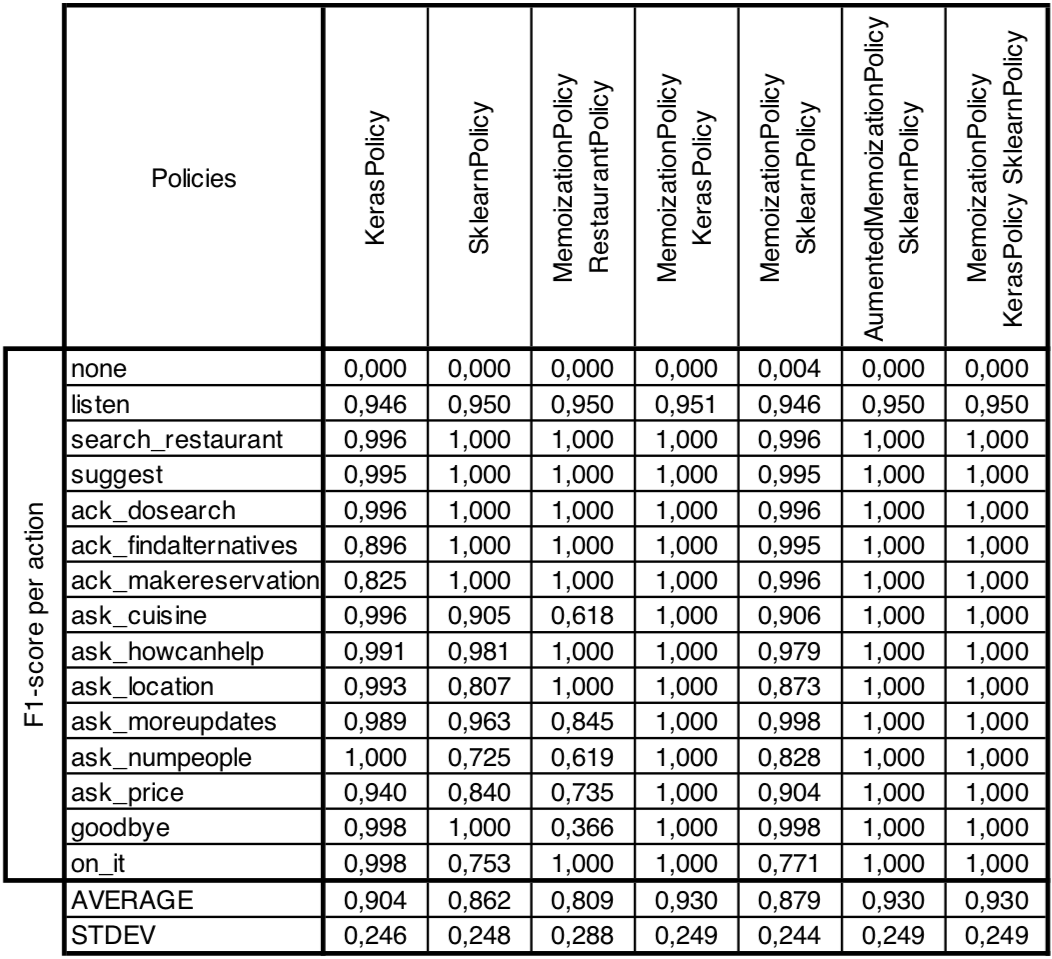
\includegraphics[scale=0.22]{core_results}
  \caption{Core results}
  \label{fig:results2}
\end{figure}

The RestaurantPolicy is a variant of the KerasPolicy, with a different model architecture. The results for different combinations of policies are showed in figure \ref{fig:results2}. Given the low performances of some policies like FallbackPolicy (even if combined with some others) their results are not reported because not really interesting. As can be seen from the results table, there are some combinations of policies that perform really well. Has to be taken into account that Sklearn policies are very fast to be trained and evaluated with respect to Keras ones, and that the performances of Sklearn + AugmentedMemoization are very similar to the ones of Keras + Memoization. This confirms that the better combination of policies between our trials is Sklearn + AugmentedMemoization. The rare errors are mainly due to the listen action being exchanged for the do-nothing action (None).

\section{Conclusions}

First, some considerations about the performances of Rasa NLU and the policies of rasa Core. Both performs very well, thanks to the two datasets that have a high quality and very few errors and thanks to the small sets of intents, entities and actions that have to be predicted. The combination of this components with the two libraries for TTS and STT and with a big database, gives the possibility to make a reservation of a restaurant using really only the voice (and some patience). However there are some improvement that should be applied for a better experience and real applications, in particular:
\begin{itemize}
\item Increase the number of possible responses of the bot, possibly implementing some natural language generator. This will create a more human-like Bot and will be more appreciated by users.
\item Increase the number of filters a user can apply when asking for restaurants.
\item Decrease the time needed by the Bot to start listening after having said something to the user.
\end{itemize}
Finally, what we can say is that this first approach has a big potential and more complex and refined model can be created on it. Like other applications of machine learning, the main problem will not be to write code but to retrieve big datasets to train custom models and evaluate them.

A complete example of the code is available here: \url{https://github.com/Luca1995it/LUS-project2}

\bigskip


\begin{thebibliography}{2}

\bibitem{pipeline}
Pipeline of RasaNLU \\
\url{https://nlu.rasa.com/pipeline.html}

\bibitem{speech_study}
Study about the performances of some speech recogniser services \\
\url{https://www.cs.montana.edu/izurieta/pubs/sede2_2015.pdf}

\bibitem{rasa_core}
Rasa Core documentation \\
\url{https://core.rasa.com/index.html}

\bibitem{rasa_nlu}
Rasa NLU documentation \\
\url{https://nlu.rasa.com/index.html}

\end{thebibliography}

\end{document}
